% Compiler ce document 

% package de base
\documentclass[10pt,a4paper]{article}
\usepackage[utf8]{inputenc}
\usepackage{listings}

% langues
\usepackage[usenames,dvipsnames]{xcolor}
\usepackage[francais]{babel}
\usepackage[T1]{fontenc}
\usepackage{amsmath}
\usepackage{amsfonts}
\usepackage{amssymb}
\usepackage{graphicx}
\usepackage{tabularx}
\usepackage{colortbl}
\usepackage[hyphens]{url}
\usepackage[hidelinks]{hyperref} % liens
\usepackage{fancyhdr} % En tetes / bas de page
\usepackage{helvet} % police helvetica
\usepackage{xcolor} % Style pour affichage du C
\usepackage{courier} % police pour les listings

\usepackage{listingsutf8}

% Page de Garde -- Necessite d'installer le package titling, si probleme
% commenter la ligne suivante ainsi que les infos necessaires a la page
% de garde
\usepackage{pageGarde/Garde_perso}

% commande pour faire des sections sans nombre 
% tout en la rajoutant dans la table des matières
\newcommand\sectionWithoutNumber[1]{\section*{#1} \addcontentsline{toc}{section}{\protect\numberline{}#1}}
\newcommand\subsectionWithoutNumber[1]{\subsection*{#1} \addcontentsline{toc}{subsection}{\protect\numberline{}#1}}
\newcommand\subsubsectionWithoutNumber[1]{\subsection*{#1} \addcontentsline{toc}{subsubsection}{\protect\numberline{}#1}}
% définition de nouvelles couleurs
\definecolor{lightblue}{rgb}{0.8,0.8,0.9}
\definecolor{grossblue}{rgb}{0,0,0.7}
%marge des pages
\setlength{\textwidth}{16cm}
\setlength{\textheight}{24cm}
\setlength{\oddsidemargin}{0cm}
\setlength{\voffset}{-1.5cm}
\setlength{\headheight}{15pt}

% set la police en arial
%% Sans-serif Arial-like fonts
\renewcommand{\rmdefault}{phv} 
\renewcommand{\sfdefault}{phv} 
\usepackage{tabularx}
\usepackage{graphicx}
\usepackage{eurosym}
\usepackage{xspace}
\newcommand{\projectname}[0]{LTANR\xspace} 

% configuration pour des listings
\lstset{ 
  showspaces=false,      
  showstringspaces=false, 
  showtabs=false,               
  tabsize=3,                     
  numbers=left
}

%enlève indentation en début de paragraphe
\setlength\parindent{0pt}

%style de l'en-tête de page
\pagestyle{fancy}

% style pour code en c
\lstdefinestyle{customc}{
  belowcaptionskip=1\baselineskip,
  breaklines=true,
  frame=L,
  xleftmargin=\parindent,
  language=C,
  showstringspaces=false,
  basicstyle=\scriptsize\ttfamily,
  keywordstyle=\bfseries\color{green!40!black},
  commentstyle=\itshape\color{purple!40!black},
  identifierstyle=\color{blue},
  stringstyle=\color{orange},
}

\lstdefinelanguage{VHDL}{
      morekeywords=[1]{
        library,use,all,entity,is,port,in,out,end,architecture,of,
        begin,and,or,Not,downto,ALL
      },
      morekeywords=[2]{
        STD_LOGIC_VECTOR,STD_LOGIC,IEEE,STD_LOGIC_1164,
        NUMERIC_STD,STD_LOGIC_ARITH,STD_LOGIC_UNSIGNED,std_logic_vector,
        std_logic
      },
      morecomment=[l]--
    }
    \usepackage[usenames,dvipsnames]{xcolor}
    \colorlet{keyword}{blue!100!black!80}
    \colorlet{STD}{Lavender}
    \colorlet{comment}{green!80!black!90}
    \lstdefinestyle{vhdl}{
      language     = VHDL,
      basicstyle   = \footnotesize \ttfamily,
      keywordstyle = [1]\color{keyword}\bfseries,
      keywordstyle = [2]\color{STD}\bfseries,
      commentstyle = \color{comment}
      breaklines=true,                % sets automatic line breaking
      tabsize=3                                % sets default tabsize to 2 spaces
    }

\lstset{escapechar=@,style=customc}
\lstset{inputencoding=utf8/latin1} %affiche les accents dans le listing

% Mise en forme de la page de titre
\author{João Miguel Domingues Pedrosa \\ Loïc Haas}
\title{Threading Building Blocks}
\dest{}

% Informations necessaires a la page de garde
% Commenter si probleme de compilation
\acro{HPC}
\matter{High Performance Coding}
\date{\today}

%en-tête
\lhead{Domingues \& Haas}
\chead{TBB}
\rhead{\theAcro}

%pied-de-page
\lfoot{HEIG-VD}
\cfoot{\today}
\rfoot{\thepage}

\begin{document}
\maketitle
\newpage
\tableofcontents
\newpage

%Ici commence réelement l'écriture du rapport

\section{Introduction}
L'objectif de ce projet est de comprendre, essayer et exploiter un outil d'optimisation. Dans notre cas, nous avons choisi TBB (Threading Building Blocks). Il s'agit d'une libraire d'Intel fait pour du C++. \\

Sa caractéristique est de simplifier au maximum l'implémentation de programme parallèle pour des systèmes multicœur. Le développeur pourra ainsi faire un programme portable car c'est la librairie qui va se charger d'utiliser la bonne implémentation de thread (exemple: POSIX pour linux ou les threads Windows). Pour cela, elle met en place différentes fonctions et classes lié à la programmation parallèle et à la gestion de concurrence.\\

Pour ce projet, nous avons du faire l'installation de la libraire, la procédure sera expliqué plus loin dans le document. Il y aura aussi un code exemple auquel on aura fait des mesures de performances afin de voir les optimisation apporté. Nous finirons par une analyse de notre constats tout au long de nos essaies.
\newpage

\section{Installation}
L'installation des libraires a été fait sur des machines possédant un OS Linux Ubuntu. Les installations suivantes ont été fait via ligne de commande.

\subsection{Installation via gestionnaire de package}

Pour installer sur nos machines, nous avons utilisé le gestionnaire de package \texttt{apt-get}. Le package installé est \texttt{libtbb2}. Nous avons donc la commande suivante pour installer:\\

\texttt{sudo apt-get install libtbb2}\\

Une fois installé, on peut commencer à programmer avec les librairies pthreads. Pour tester l'installation, on va compiler et exécuter un code exemple afin de voir s'il n'y a pas de problème.(commande pour la compilation \texttt{g++ <filename>.cpp -ltbb} )

\subsubsection{Code exemple}
\lstinputlisting{../test/test.cpp}

\newpage

\subsection{Installation via l'archive}

\begin{enumerate}

	\item Il faut premièrement télécharger. Pour cela, il faut se rendre sur le site d'Intel pour TBB et aller dans la section download\footnote{\url{https://www.threadingbuildingblocks.org/download}}. Ensuite, on copie l'adresse sur la release et l'OS que l'on veut (dans notre cas Linux). On entre ensuite la commande suivante:\\
	\texttt{\$ wget https://www.threadingbuildingblocks.org/sites/default/files/\linebreak software\_releases/linux/tbb<version>.tgz}
	
	\item Maintenant que l'on a télécharger l'archive, il faut l'extraire pour cela on fait la commande suivante:\\
	\texttt{\$ tar zxf tbb<version>.tgz}
	\item Un fois extrait, il faut se rendre dans le dossier \texttt{bin} et modifier le script \texttt{tbbvars.sh}. Il faut changer la ligne suivante:\\
	\texttt{TBBROOT = SUBSTITUTE\_INSTALL\_DIR\_HERE} \\
	par\\
	\texttt{TBBROOT = <path\_tbb\_directory>}\\
	Cela permettra alors de pouvoir utiliser la librairie facilement lors de la compilation.
	\item Après, on exécute le script avec la bonne option (ia32 pour une architecture 32 bits ou intel64 pour du 64 bits) et on peut commencer à faire des programmes avec TBB.
	\item Pour tester si tout a été bien installé, on compile le code précédent et on l'exécute.
	Si il n'y a pas eu de problème durant la compilation et l'exécution c'est que tout est bon
\end{enumerate}

\begin{figure}[hpl]
	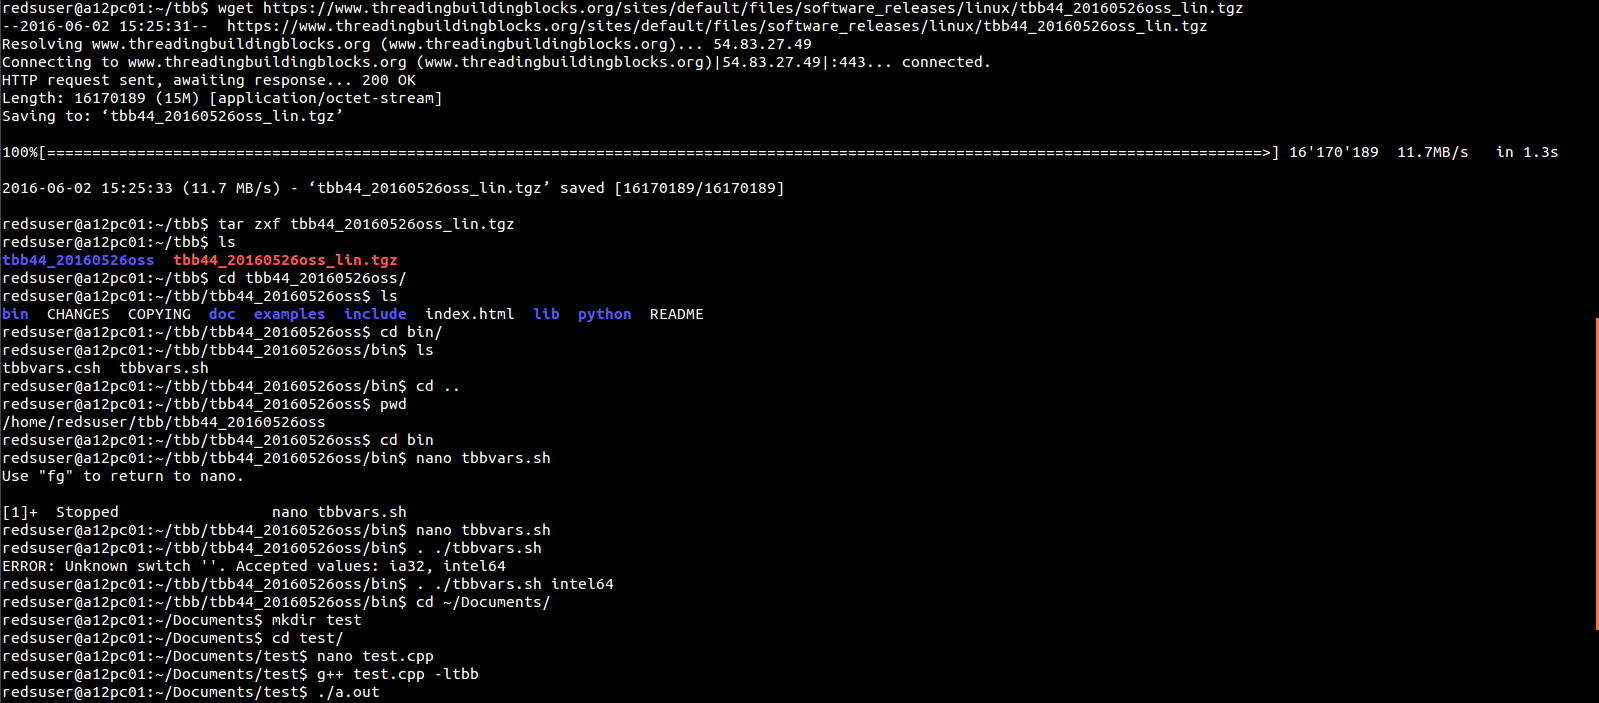
\includegraphics[width=\textwidth]{images/installcommands.png}
	\caption{Capture d'écran des commandes utilisées}
\end{figure}

\newpage

\section{Exemple}
Le programme utilisé pour l'exemple s'occupe de compter le nombre d’occurrence des caractères de la table ASCII.Nous avons choisi le code suivant car il se prête bien à la parallélisation et que nous avons déjà fait une implémentation parallèle avec les thread POSIX directement et en C. Cela nous permet ainsi de faire des meilleurs critiques au niveau des performances.\\

Commande pour la compilation: \texttt{g++ -O3 -std=c++11 statscount.cpp -o statscount -ltbb}

\subsection{Code}
% inserer le code ici
\lstinputlisting{../examples/stats_count/statscount.cpp}

\subsubsection{Explication}
La libraire TBB possède beaucoup de fonction permettant le parallélisation. Pour expliquer le fonctionnement, nous allons montrer comment fonctionne une d'elle, le \texttt{paralle\_for}. \\

Cette fonction possède plusieurs entête différents qui varie selon ce qu'on a besoin. Ici, on utilise une qui demande une classe template \texttt{blocked\_range} et une expression lambda. L'expression lambda correspondra à la fonction que devront effectuer chaque thread lancé par le programme. Ici, il s'agit de compter le nombre d’occurrences de chaque caractère dans un fichier. 

La classe \texttt{blocked\_range} permet la répartition de l'exécution du programme dans tout les cœurs du système. Il faut lui indiquer dans le constructeur la range d'itérations qu'il y a maximum à faire, 0 à n-1. Cela permettra dans les boucles for interne, ou autre calcul nécessitant la connaissance des index, d'utiliser le \texttt{begin} et \texttt{end} afin de pouvoir bien répartir les données. Cela est utile quand certaine partie prenne plus de temps que d'autre. Ainsi, lorsqu'un thread se termine on lance directement dessus le jeux de données suivant.
Cela abstrait la répartition des données manuel dans chaque thread et l'optimisant sachant que l'on attend sur le thread le plus rapide. Dans notre exemple, on utilise se procédé pour mettre le pointeur de fichier au bonne endroit selon les threads:
\lstinputlisting[firstline=44, lastline=45]{../examples/stats_count/statscount.cpp}
On l'utilise aussi dans la boucle for qui va lire le fichier:
\lstinputlisting[firstline=53, lastline=58]{../examples/stats_count/statscount.cpp}

\newpage

Une autre variante de \texttt{parallel\_for} exige comme paramètre un min, un max, un step et une fonction (ou expression lambfa). Celle-ci diffère de l'autre par le paramètre step. Il s'agit au fait du nombre de pas qui sépare chaque itérations de thread. Par exemple, on veut itère de 0 à n-1 mais on veut le faire que sur les nombres pair, donc un sur deux. Il suffit de mettre un step de 2 et on aura la réaction voulu. La répartition des tâches sera la même que le \texttt{parallel\_for} discuté avant mais on aura moins d'itérations et l'index fournit sera calculer selon ce paramètre. Exemple:\\
Série:

\begin{lstlisting}
for(int i=0; i < N-1; i+=2){
	tabPair[i/2] = i;
}
\end{lstlisting}

Parallèle TBB:

\begin{lstlisting}
parallel_for(0, N-1, 2, [tabPair](const int& i) {
	tabPair[i/2] = i;
});
\end{lstlisting}


Ensuite, pour récolter le nombre d'occurrences dans chaque de caractères que possède chaque thread, on passe par une classe template combine. Cette classe demande une expression lambda au constructeur:
\lstinputlisting[firstline=17, lastline=17]{../examples/stats_count/statscount.cpp}
Cela va générer un objet du type voulu lors du lancement du thread. On pourra le récupérer à chaque fois que l'on appelle la méthode \texttt{local} de la classe, on renvoi un vecteur d'une certaine taille dans notre cas:
\lstinputlisting[firstline=51, lastline=51]{../examples/stats_count/statscount.cpp}
Il va s'agir ici de Thread Local Storage. Cela veut dire que tout les threads possède le même objet qui se trouve à la même plage d'adresse mais qui est indépendant pour chaque thread et donc que son contenu est différent. Dans notre cas, on aimerait qu'à la fin, on est un seul tableau et non plusieurs contenant le nombre total d’occurrences pour chaque caractère. Pour cela, une fois l'exécution du \texttt{parallel\_for} terminé, on appelle la méthode \texttt{combine\_each} et on lui passe  une expression lambda récupérant le nombre d'occurrences rencontré pour chaque thread dans un seul tableau:
\lstinputlisting[firstline=67, lastline=72]{../examples/stats_count/statscount.cpp}
La même chose est fait pour la répartition du fichier. On applique un \texttt{close} en fin d'exécution:
\lstinputlisting[firstline=74, lastline=78]{../examples/stats_count/statscount.cpp}

\newpage

\subsection{Équivalent C}

\lstinputlisting{../examples/stats_count/statscount.c}

\subsection{Remarque}
On voit que la version C++ TBB est plus élégante que la version C POSIX. Dans la version C, il faut préparer tout les threads leur définir la taille de données, où sa commence et où il faut s'arrêter. De plus, c'est nous qui devons choisir nous même le nombre de thread. Alors que TBB, lui, choisi tout seul le nombre de thread optimum à lancé.

\subsection{Mesures}
Les mesures ont été effectué sur un fichier d'environ 250 MB. On a utilisé l'utilitaire \texttt{perf} afin de relever des données intéressante sur les performances de notre implémentation TBB.

Commande utilisé: \texttt{perf stat -e task-clock,cycles,instructions,cache-references,cache-misses <exec> <filepath> }

\subsubsection{TBB}
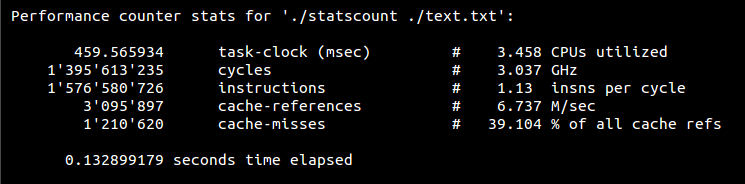
\includegraphics[scale=0.5]{images/perf_tbb}


\subsubsection{POSIX}
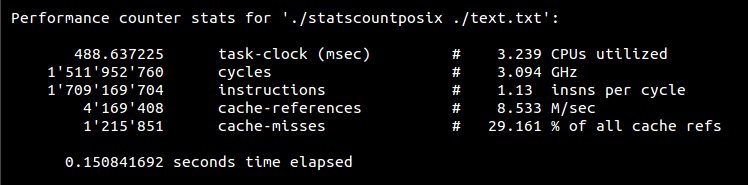
\includegraphics[scale=0.5]{images/perf_posix}
\newpage

\section{Analyse}
On peut qu'entre la version TBB et POSIX, la différence est moindre. On a juste quelque problème au niveau de la cache avec TBB mais on arrive pas comme ça à identifier d'où vient le problème. Par contre, on voit bien que les CPUs sont bien utilisé dans les deux cas. On a plus que 3 CPU utilisé durant l’exécution du programme. On peut donc dire que TBB fait bien sont travaille et parallélise notre implémentation.

\section{Conclusion}
Au final, on voit que la librairie TBB fait bien sont travaille. Elle repartit la tâche dans plusieurs threads et dans tout les coeurs sans même avoir à demander combien de thread on veut lancer. Il exploite ainsi tout le potentiel de processeur sans que le développeur est à se soucier combien de thread il doit lancer. On a donc une bonne abstraction de la part de la librairie avec des performances satisfaisante qui permet au développeur de faire du code simple, compréhensible et générique, sachant que la libraire s'adapte tout seul à l'implémentation des threads selon l'OS ou l'architecture utilisé.

\section{Bibliographie}
\begin{itemize}
	\item Tutoriel d'Intel: \url{https://www.threadingbuildingblocks.org/intel-tbb-tutorial}
	\item Documentation d'Intel: \url{https://software.intel.com/en-us/tbb-documentation}
	\item Présentation d'Intel: \url{http://www.cs.cmu.edu/afs/cs/academic/class/15499-s09/www/handouts/TBB-HPCC07.pdf}
\end{itemize}

\end{document}
